\chapter{Metodologia}
\label{cap:metodologia}

\section{Microsserviços}

    O VuMoS foi implementado utilizando uma arquitetura modular de microsserviços, para que ele possa ser facilmente estendido e modificado no futuro caso necessário, e também para proporcionar uma maior facilidade de desenvolvimento de cada um dos módulos.
    
    Estes microsserviços usam um sistema de troca de mensagems como base para comunicação entre si, facilitando a comunicação assíncrona entre eles. Tal sistema também facilita o envio de mensagens de \textit{broadcast}, para que informações de um dos módulos chegue em diversos outros módulos enviando-as apenas uma vez. 
    
    % TODO: falar de Publish/subscribe?
    
    \subsection{NATS}
    
    Foi escolhido o NATS\footnote{\url{https://nats.io}} como o sistema de mensageria da aplicação, principalmente devido a sua escalabilidade, simplicidade e performance. Ele envia mensagens do tipo JSON através de um socket TCP, e portanto pode ser facilmente integrado em diversas arquiteturas e linguagens de programação. Além disso, as principais delas já contam com bibliotecas que implementam o protocolo NATS em seus repositórios (como Pipy\footnote{\url{https://pypi.org/project/asyncio-nats-client/}} e NPM\footnote{\url{https://www.npmjs.com/package/nats}}, por exemplo).
    
    
\section{Módulos}
    
    O sistema foi projetado para que cada módulo possa ser implementado em qualquer linguagem de programação, e usando qualquer paradigma, desde que ele seja capaz de se comunicar com o sistema de mensageria NATS e siga o protocolo de mensagens especificado. Este protocolo foi definido no repositório \textit{common} usando \textit{json-schema}\footnote{\url{https://json-schema.org/}}, já que uma mensagem no NATS é enviada no formato JSON. 
    
    \begin{figure}
        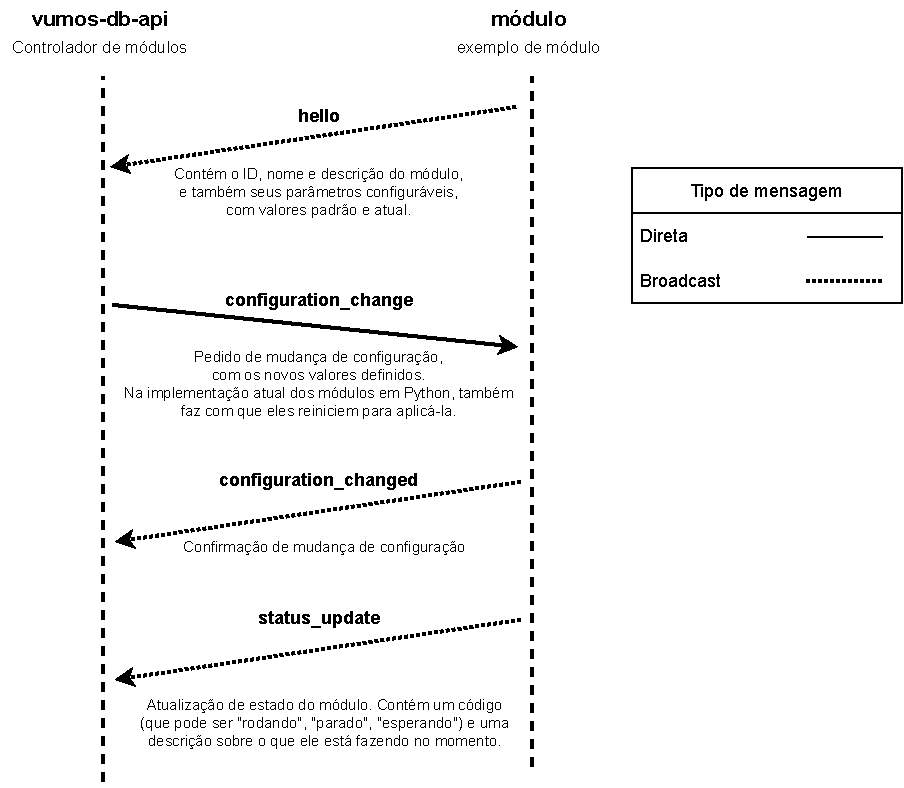
\includegraphics[scale=0.8]{figuras/vumos-module-communication.drawio.pdf}
        \caption{Diagrama de troca de mensagens entre um módulo e o gerenciador vumos-db-api.\label{fig:module-communication}}
    \end{figure}
    
    Como exemplificado em \ref{fig:module-communication}, quando um módulo é inicializado ele envia uma mensagem do tipo \textit{hello}, que anuncia sua presença aos outros módulos do
    sistema. Essa mensagem contém o \textit{VUMOS\_ID} (que corresponde a um 
    \textit{uuid} que representa o módulo), nome e descrição do 
    módulo, e também quais são seus parâmetros configuráveis. Nessa mensagem também são enviados os valores padrão de tais configurações.

    
    \begin{figure}
        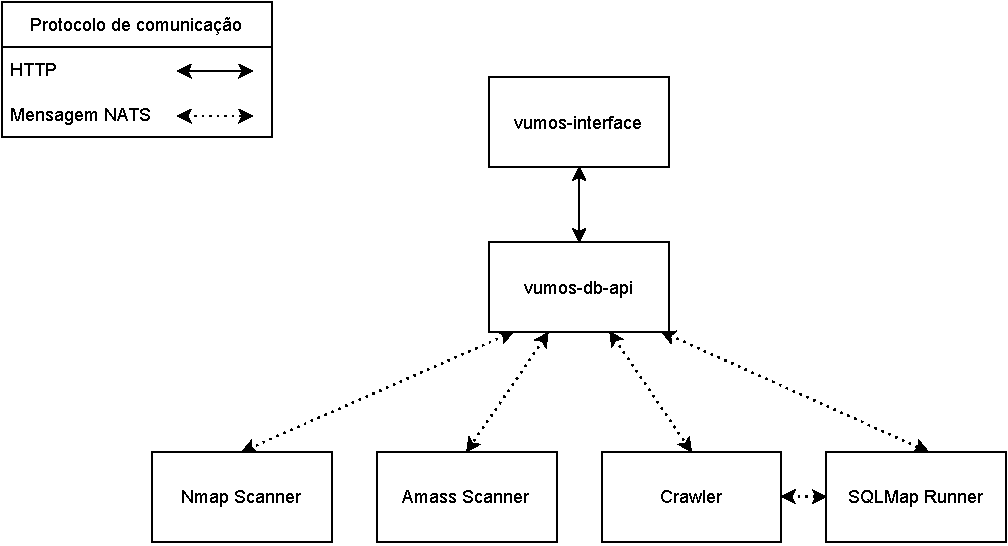
\includegraphics[scale=0.8]{figuras/vumos-Microservices.pdf}
        \caption{Diagrama de comunicação dos microsserviços implementados.\label{fig:microservices}}
    \end{figure}
    
    Além disso, módulos podem interagir entre si de maneiras distintas quando necessário, como é o caso do Crawler e do SQLMap Runner.
    
    \subsection{Vumos Common}
    Seguindo a arquitetura de microsserviços, cada módulo é responsável pelo armazenamento das informações relevantes a seu funcionamento, podendo ser elas obtidas através do prório módulo ou através de mensagens recebidas por outros módulos. 
    
    Para facilitar o processo de desenvolvimento de um novo módulo, foi implementada uma biblioteca em \textit{Python} que funciona como arcabouço para os outros módulos, e também contém o \textit{schema} das mensagens da aplicação.
    
    Ele conta com um banco de dados local implementado em SQLite, usado principalmente para o armazenamento das configurações do módulo. Para facilitar o seu acesso do ponto de vista do desenvolvedor, foi implementado um conjunto de funções que tornam o seu uso transparente.
    
    Para que seja possível enviar e receber mensagens do módulo enquanto ele executa outras tarefas, como escrita no banco de dados ou requisições HTTP, foi utilizada uma arquitetura de computação assíncrona, utilizando a biblioteca \textit{asyncio} do Python. Isso nos proporciona métodos interessantes para a execução de subprocessos, o que é necessário para uma grande parte dos módulos a serem implementados, além de proporcionar um maior desempenho no que se diz respeito a esse tipo de operação. 
    
    \subsection{Amass Scanner}
    
    Este módulo tem como objetivo encontrar subdomínios existentes no domínio principal \url{usp.br}, usando para isso a ferramenta de código aberto AMASS \footnote{\url{https://github.com/OWASP/Amass}}. Esta ferramenta utiliza diversas técnicas de enumeração de DNS para tentar encontrar subdomínios válidos, sendo algumas delas:
    \begin{itemize}
        \item \emph{Força bruta}: São testados diversos nomes comuns de subdomínios em um servidor de DNS para verificar se algum deles está disponível no domínio da USP.
        \item \emph{Scraping}: O domínio principal é buscado num motor de busca existente (como Google ou DuckDuckGo) e os subdomínios encontrados são adicionados à lista.
        \item \emph{Certificados}: São verificados os valores válidos para subdomínios encontrados nos certificados TLS fornecidos pelos servidores HTTP rodando no domínio principal.
        \item \emph{Páginas arquivadas}: São buscados subdomínios em páginas arquivadas por serviços como ArchiveIt\footnote{\url{https://archiveit.com/}} ou WaybackMachine\footnote{\url{https://web.archive.org/}} para encontrar subdomínios que não estão mais publicamente acessíveis, mas ainda podem ser válidos.
    \end{itemize}
    
    A unica variável configurável deste módulo é o domínio inicial que será escaneado.
    
    Uma vez encontrados os subdomínios, é enviada uma mensagem como \textit{broadcast} com os tal informação em seus respectivos hosts/alvos.
    % TODO: link com vumos-db-api falando dos targets?
    \subsection{Nmap Scanner}
    Este módulo tem como objetivo encontrar máquinas na rede e seus serviços, obtendo também informações sobre eles, como em quais portas estão rodando, quais versões, e possivelmente se possuem alguma vulnerabilidade conhecida. Para isso, é utilizada a ferramenta de código aberto de mapeamento de rede NMAP \footnote{\url{https://github.com/OWASP/Amass}}, que realiza todas essas funções para cada um dos IPs que ela encontra.
    
    Como variáveis configuráveis deste módulo, temos:
    \begin{itemize}
        \item \emph{Flags}: São os argumentos de linha de comando que serão enviados ao NMAP, ativando ou desativando cada uma de suas features. Por exemplo, aqui podemos ativar ou desativar a busca automatizada por vulnerabilidades conhecidas.
        \item \emph{Redo Days}: Quantidade de dias até que o escaneamento seja realizado novamente
        \item \emph{IP Ranges}: Quais IPs serão escaneados. São aceitos IPs no formato \textit{CIDR Standard} separados por vírgula, ou seja, é possível definí-lo para escanear todas as subredes da USP de uma vez.
    \end{itemize}
    
    Por fim, para cada serviço encontrado é enviada uma mensagem como \textit{broadcast} e também é enviada uma mensagem com seu alvo.
    
    \subsection{Crawler}
    Este módulo tem o objetivo de, a partir de uma página HTML inicial, encontrar novas páginas que possuem links dinâmicos. Isso é feito usando um \textit{crawler} customizado que utiliza o módulo de Python Scrapy \footnote{\url{https://scrapy.org/}}. Como não é possível saber se um link é processado dinamicamente ou não pelo servidor sem uma análise extensa em cada um deles, é utilizada uma heurística, que nos permite conseguir uma grande quantidade de links dinâmicos sem processamento extra. Portanto, uma URL é considerada dinâmica se contiver uma interrogação (indicando que contém parâmetros, sendo eles analisados para uso futuro), ou se for o resultado de um envio de formulário, onde os parâmetros são seus campos. 
    
    Como variáveis configuráveis deste módulo, temos:
    \begin{itemize}
        \item \emph{Allowed domains}: Domínios onde o crawler é permitido a rodar. Isso impede que domínios fora do escopo sejam escaneados quando um link externo (como do Youtube, por exemplo) for encontrado.
        \item \emph{Initial URLs}: Lista separada por vírgulas com as URLs por onde o crawler começará a procurar links. 
    \end{itemize}
    
    Para cada URL dinâmica encontrada, é enviada uma mensagem como \textit{broadcast} e também é enviada uma mensagem com seu alvo e com seu serviço, sendo tais informações extraidas tanto da URL em si quanto da página que a contém.
    
    \subsection{SQLMap Runner}
    Este módulo tem como objetivo procurar vulnerabilidades de SQL Injetion em uma determinada URL dinâmica através da ferramenta de código aberto SQLMap \footnote{\url{https://github.com/sqlmapproject/sqlmap}}. Para isso, este módulo escuta pelas mensagens de \textit{broadcast} do tipo \textit{Path}, que são enviadas pelo módulo do Crawler e, para cada uma delas, coloca numa fila persistente em disco. Isso é feito pois o SQLMap, devido à sua complexidade, demora diversas vezes mais para ser executado em relação ao Crawler, portanto as URLs são acumuladas nesta fila e processadas assim que possível.
    
    Para tornar o processo mais rápido, este módulo implementa também um sistema de \textit{multithreading}, no qual diversas instâncias do SQLMap são executadas ao mesmo tempo em URLs diferentes para paralelizar o processo. Para tal, foi utilizado o gerenciamento de \textit{threads} de execução do \textit{asyncio}, onde cada instância do SQLMap é iniciado em uma co-rotina assíncrona com um executor próprio.
    
    Para buscar tais vulnerabilidades, o SQLMap executa diversas requisições HTTP com alterações em seus parâmetros, e verifica por diferenças nos resultados, de acordo com as seguintes técnicas:
    
    \begin{itemize}
        \item \emph{Boolean-based blind}: Em português "ataque cego baseado em booleanos", esta técnica adiciona parâmetros de SQL válidos na requisição HTTP, e para 
        
        sqlmap replaces or appends to the affected parameter in the HTTP request, a syntatically valid SQL statement string containing a SELECT sub-statement, or any other SQL statement whose the user want to retrieve the output. For each HTTP response, by making a comparison between the HTTP response headers/body with the original request, the tool inference the output of the injected statement character by character. Alternatively, the user can provide a string or regular expression to match on True pages. The bisection algorithm implemented in sqlmap to perform this technique is able to fetch each character of the output with a maximum of seven HTTP requests. Where the output is not within the clear-text plain charset, sqlmap will adapt the algorithm with bigger ranges to detect the output.
    \end{itemize}
    
    Como variáveis configuráveis deste módulo, temos:
    \begin{itemize}
        \item \emph{Number of instances}: Quantidade de instâncias do SQLMap que serão executadas ao mesmo tempo.
        \item \emph{SQLMap Techniques}: Lista separada por vírgulas com as URLs por onde o crawler começará a procurar links. 
    \end{itemize}


    \subsection{vumos-db-api}
        % TODO: falar do DB, postgres e mostrar um diagrama
    \subsection{vumos-interface}
        % TODO: botar uns prints bonitinhos
    

\section{Orquestração}
    
    % TODO: falar das networks 
    \subsection{Produção}
    O VuMoS foi colocado em produção em http://vumos.hackersdobem.sti.usp.br/ e já está atualmente escanenado os  

% TODO: falar da organização dos repositórios





% 